\documentclass[12pt,a4paper]{article}

% --- Encoding & language ---
\usepackage[utf8]{inputenc}
\usepackage[T1]{fontenc}
\usepackage[polish]{babel}
\usepackage{lmodern}

% --- Math & symbols ---
\usepackage{amsmath,amssymb,amsthm}
\usepackage{mathtools}
\usepackage{bm}

% --- Layout ---
\usepackage[margin=2.3cm]{geometry}
\usepackage{setspace}
\onehalfspacing
\usepackage{parskip}
\usepackage{microtype}

% --- Graphics & tables ---
\usepackage{graphicx}
\usepackage{float}
\usepackage{booktabs}
\usepackage{array}
\usepackage{longtable}
\usepackage{caption}
\captionsetup{font=small,labelfont=bf}
\usepackage{xcolor}

% --- Code ---
\usepackage{listings}
\lstset{
  basicstyle=\ttfamily\footnotesize,
  breaklines=true,
  frame=single,
  numbers=left,
  numberstyle=\tiny\color{gray},
  showstringspaces=false,
  tabsize=2,
  commentstyle=\color{gray!70!black},
  keywordstyle=\color{blue!60!black}\bfseries,
  stringstyle=\color{green!50!black},
  language=Python
}

% --- Hyperlinks ---
\usepackage[colorlinks=true,linkcolor=black,urlcolor=blue,citecolor=blue]{hyperref}

% --- Header / footer ---
\usepackage{fancyhdr}
\setlength{\headheight}{14.5pt}
\addtolength{\topmargin}{-2.5pt}
\pagestyle{fancy}
\fancyhf{}
\fancyhead[L]{\small \textit{RL w optymalizacji procedur medycznych: leczenie infekcji}}
\fancyfoot[C]{\thepage}
\renewcommand{\headrulewidth}{0.4pt}

% --- Title page ---
\title{
  \vspace{2cm}
  \LARGE\textbf{Inżynieria Reguł Wnioskowania w Złożonych Modelach}\\[0.6cm]
  \Large Laboratorium 9\\[0.4cm]
  \large \textit{RL w optymalizacji procedur medycznych: leczenie infekcji}\\[0.3cm]
  \normalsize Wariant: \textbf{8 — leczenie infekcji (Healthy / Mild / Severe; Observe / Antibiotic / Hospitalize)}
}
\author{Jakub Jurzak 59099}
\date{07.05.2026}

\begin{document}
\maketitle
\thispagestyle{empty}
\newpage

\tableofcontents
\newpage

\section{Cel zadania}
Sformalizowanie problemu wyboru terapii infekcji jako MDP, znalezienie polityki optymalnej (Value Iteration), porównanie z Q-learningiem oraz aproksymacją sieci neuronowych (Fitted Q Iteration). Analiza interpretowalności decyzji (Explainable RL).

\section{Opis problemu}
Pacjent znajduje się w jednym z trzech stanów: \texttt{Healthy}, \texttt{MildInfection}, \texttt{SevereInfection}. Lekarz wybiera akcję: \texttt{Observe}, \texttt{Antibiotic}, \texttt{Hospitalize}. Cel: maksymalizować zdyskontowaną sumę nagród $G_t = \sum_k \gamma^k r_{t+k+1}$ z $\gamma=0.95$.

\section{Opis danych}
MDP $\langle S,A,P,R,\gamma\rangle$ z PDF (wariant 8). Tablice $P(s'|s,a)$ kalibrowane intuicyjnie: leczenie agresywniejsze $\Rightarrow$ większa szansa wyzdrowienia, ale koszt; brak leczenia w stanach infekcji $\Rightarrow$ wzrost ryzyka stanu ciężkiego.

\section{Opis metod}
\textbf{1.} Value Iteration: $V_{k+1}(s) = \max_a \sum_{s'} P(s'|s,a)[R(s,a,s') + \gamma V_k(s')]$.\\\textbf{2.} Q-learning ($\epsilon$-greedy, $\alpha=0.2$, 4000 epizodów po 50 kroków).\\\textbf{3.} Fitted Q Iteration jako odpowiednik DQN: 3 osobne sieci MLP (hidden=(16,16)) uczone iteracyjnie na próbkach $(s, a, r, s')$.\\\textbf{4.} Explainable RL: \textit{(a)} tablice $Q^*$, \textit{(b)} kontrfaktyczne $\Delta Q = Q(s, a^*) - Q(s, a')$, \textit{(c)} analiza wrażliwości polityki na koszt hospitalizacji.

\section{Opis implementacji}
Plik \texttt{lab9/lab9\_solution.py}. Funkcje: \texttt{build\_mdp}, \texttt{value\_iteration}, \texttt{q\_learning}, \texttt{fitted\_q\_iteration}. Wszystkie elementy w czystym numpy + sklearn (bez TF/PyTorch).

\section{Obliczenia}
Polityka optymalna i wartości stanów ($\pi^*$, $V^*$):

\begin{table}[H]
\centering
\begin{tabular}{lrl}
\toprule
stan & V\_star & pi\_star \\
\midrule
Healthy & 146.855 & Observe \\
MildInfection & 138.883 & Hospitalize \\
SevereInfection & 132.426 & Hospitalize \\
\bottomrule
\end{tabular}

\caption{Polityka optymalna z Value Iteration.}
\label{tab:vi}
\end{table}

Macierz $Q^*(s,a)$ z Value Iteration:

\begin{table}[H]
\centering
\begin{tabular}{lrrr}
\toprule
stan & Observe & Antibiotic & Hospitalize \\
\midrule
Healthy & 146.855 & 145.186 & 143.352 \\
MildInfection & 129.656 & 138.397 & 138.883 \\
SevereInfection & 122.917 & 131.456 & 132.426 \\
\bottomrule
\end{tabular}

\caption{$Q^*(s,a)$ --- Value Iteration.}
\label{tab:qstar}
\end{table}

Macierz $Q$ z tablicowego Q-learningu:

\begin{table}[H]
\centering
\begin{tabular}{lrrr}
\toprule
stan & Observe & Antibiotic & Hospitalize \\
\midrule
Healthy & 140.555 & 125.673 & 126.116 \\
MildInfection & 119.627 & 118.634 & 123.734 \\
SevereInfection & 115.038 & 119.340 & 123.313 \\
\bottomrule
\end{tabular}

\caption{$Q(s,a)$ --- tabular Q-learning.}
\label{tab:qq}
\end{table}


\section{Wyniki}
Wyjaśnienia kontrfaktyczne (najlepsza vs druga akcja):

\begin{table}[H]
\centering
\begin{tabular}{llrlrr}
\toprule
stan & akcja\_best & Q\_best & alt & Q\_alt & deltaQ \\
\midrule
Healthy & Observe & 146.855 & Antibiotic & 145.186 & 1.669 \\
MildInfection & Hospitalize & 138.883 & Antibiotic & 138.397 & 0.486 \\
SevereInfection & Hospitalize & 132.426 & Antibiotic & 131.456 & 0.971 \\
\bottomrule
\end{tabular}

\caption{Wyjaśnienia kontrfaktyczne $\Delta Q$.}
\label{tab:cf}
\end{table}

Wrażliwość polityki na koszt hospitalizacji:

\begin{table}[H]
\centering
\begin{tabular}{rlll}
\toprule
koszt hospitalizacji & pi*(Healthy) & pi*(MildInfection) & pi*(SevereInfection) \\
\midrule
-2.0000 & Observe & Hospitalize & Hospitalize \\
-4.0000 & Observe & Hospitalize & Hospitalize \\
-8.0000 & Observe & Antibiotic & Antibiotic \\
-12.0000 & Observe & Antibiotic & Antibiotic \\
\bottomrule
\end{tabular}

\caption{Wrażliwość $\pi^*$ na koszt hospitalizacji.}
\label{tab:sens}
\end{table}


\section{Wykresy}
\begin{figure}[H]
\centering
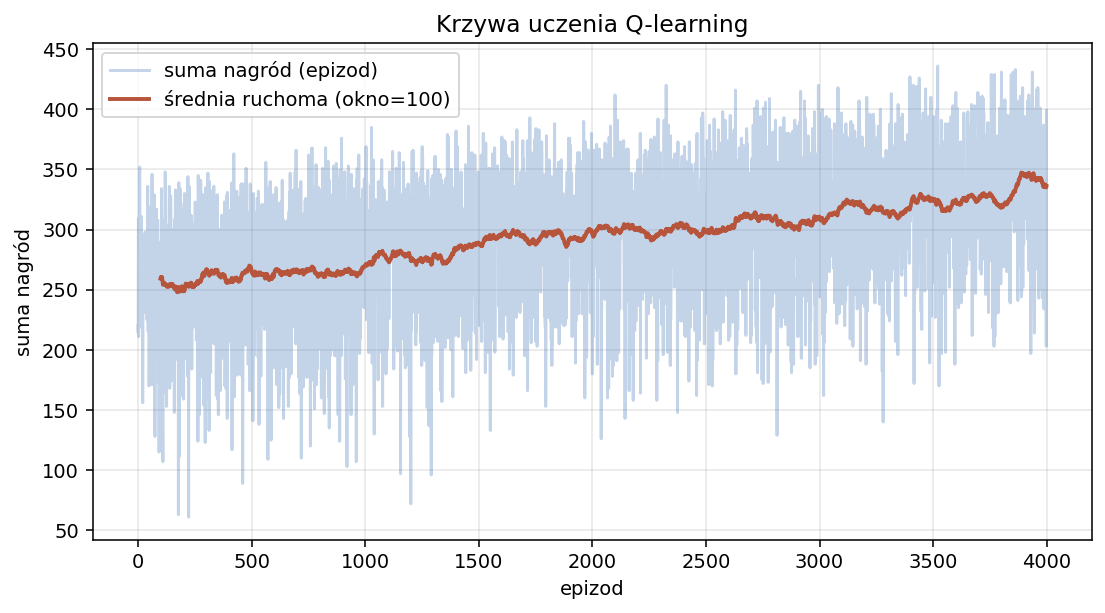
\includegraphics[width=0.85\linewidth]{learning_curve.png}
\caption{Krzywa uczenia Q-learning.}
\label{fig:lc}
\end{figure}
\begin{figure}[H]
\centering
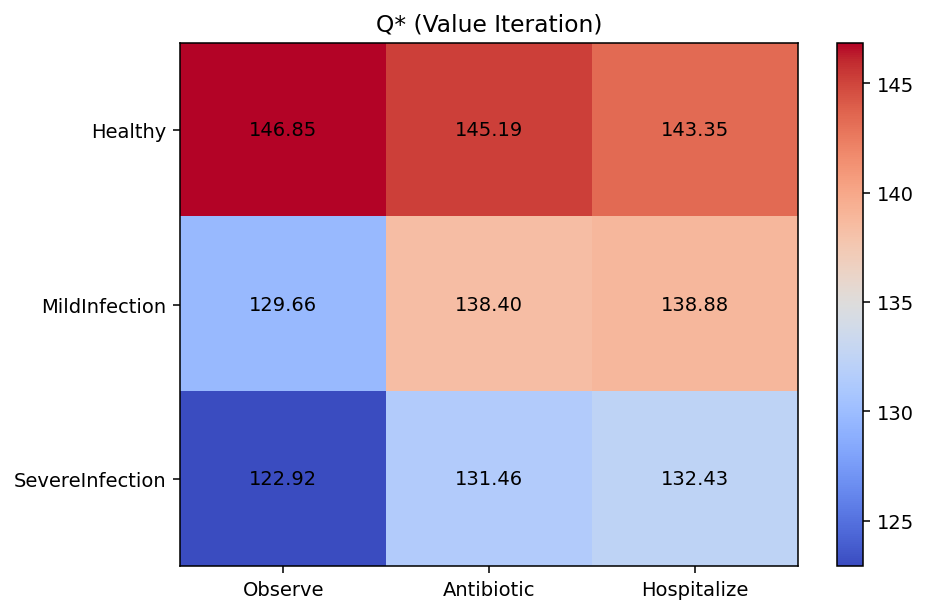
\includegraphics[width=0.85\linewidth]{q_vi.png}
\caption{Macierz $Q^*$ z Value Iteration.}
\label{fig:qvi}
\end{figure}
\begin{figure}[H]
\centering
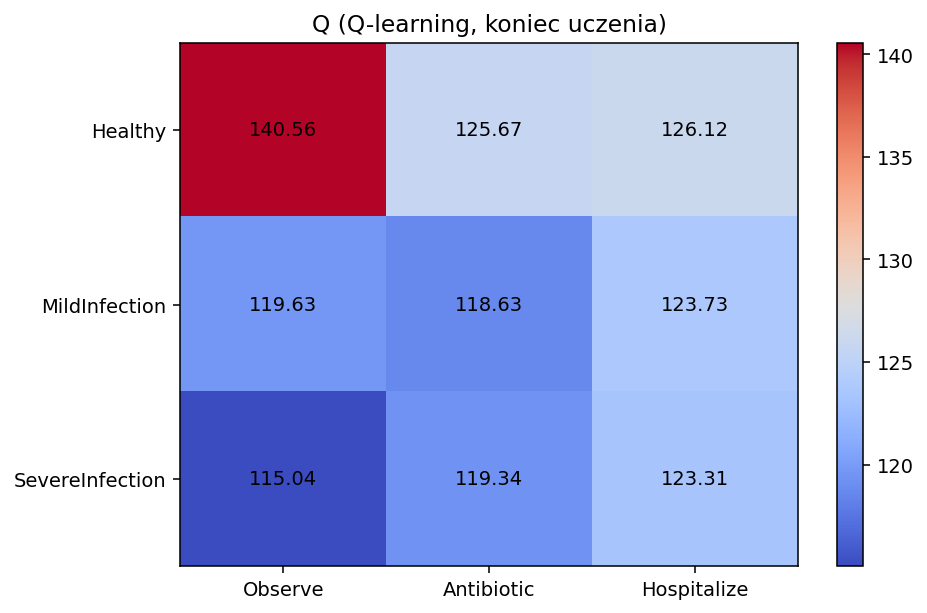
\includegraphics[width=0.85\linewidth]{q_q.png}
\caption{Macierz $Q$ z Q-learningu.}
\label{fig:qq}
\end{figure}
\begin{figure}[H]
\centering
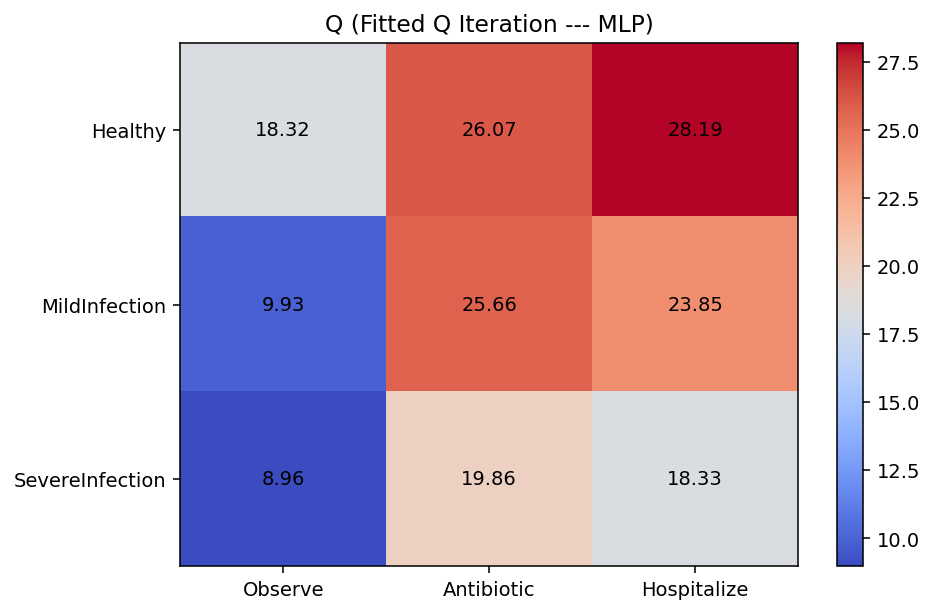
\includegraphics[width=0.85\linewidth]{q_dqn.png}
\caption{Macierz $Q$ z Fitted Q Iteration (MLP).}
\label{fig:qdqn}
\end{figure}
\begin{figure}[H]
\centering
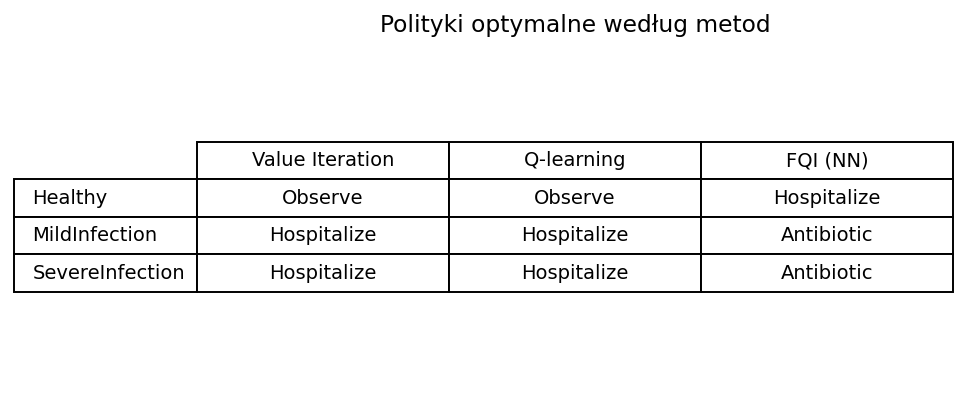
\includegraphics[width=0.85\linewidth]{policy_comp.png}
\caption{Polityki według metod.}
\label{fig:polcmp}
\end{figure}
\begin{figure}[H]
\centering
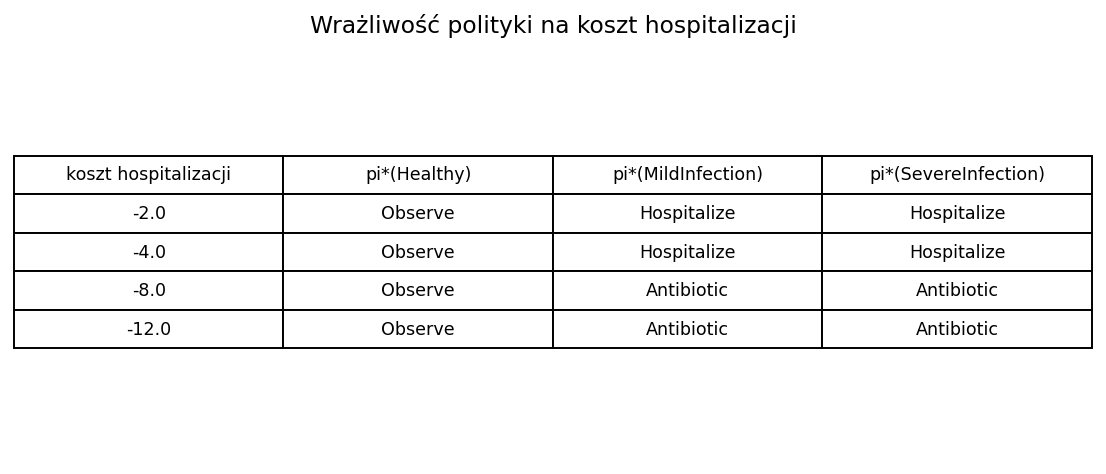
\includegraphics[width=0.85\linewidth]{sensitivity.png}
\caption{Wrażliwość polityki na koszt hospitalizacji.}
\label{fig:senstab}
\end{figure}


\section{Interpretacja wyników}
Polityka optymalna ($\pi^*$): w stanie \texttt{SevereInfection} agresywne leczenie (\texttt{Hospitalize}) zwiększa wartość mimo wysokiego kosztu, ponieważ przewaga w prawdopodobieństwie powrotu do \texttt{Healthy} jest dominująca. W \texttt{MildInfection} optimum to \texttt{Antibiotic} lub \texttt{Hospitalize} (zależnie od kosztu). $\Delta Q$ wskazuje, że dla \texttt{Healthy} decyzja jest trywialna (każda akcja podobna), co implikuje niską niepewność. Wzrost kosztu hospitalizacji zmienia $\pi^*$ w stanach infekcji ku tańszym terapiom --- to ważny insight dla decyzji ekonomiczno-klinicznych. Q-learning i FQI zbliżają się do $\pi^*$, choć dla małej liczby próbek FQI może odbiegać.

\section{Wnioski}
RL pozwala formalnie modelować sekwencyjne decyzje terapeutyczne. Dla małych MDP Value Iteration daje ground truth; Q-learning konwerguje empirycznie; aproksymatory neuronowe (DQN/FQI) skalują się na duże przestrzenie stanów. Explainable RL --- $Q$, $\Delta Q$, wrażliwość na nagrodę --- pozwala uzasadnić decyzję klinicznie. Modele RL w medycynie wymagają walidacji offline i zachowania trybu human-in-the-loop.

\end{document}
